\section{Middleware Architecture}

\subsection{Server Architecture}

The company architecture contains the following components: Client Application, Middleware server, Middleware Cache, Metadata Server, and Content Servers. The brief architecture overview is presented on figure \ref{fig:arch_overview}. 


\begin{figure}[h]
    \centering
	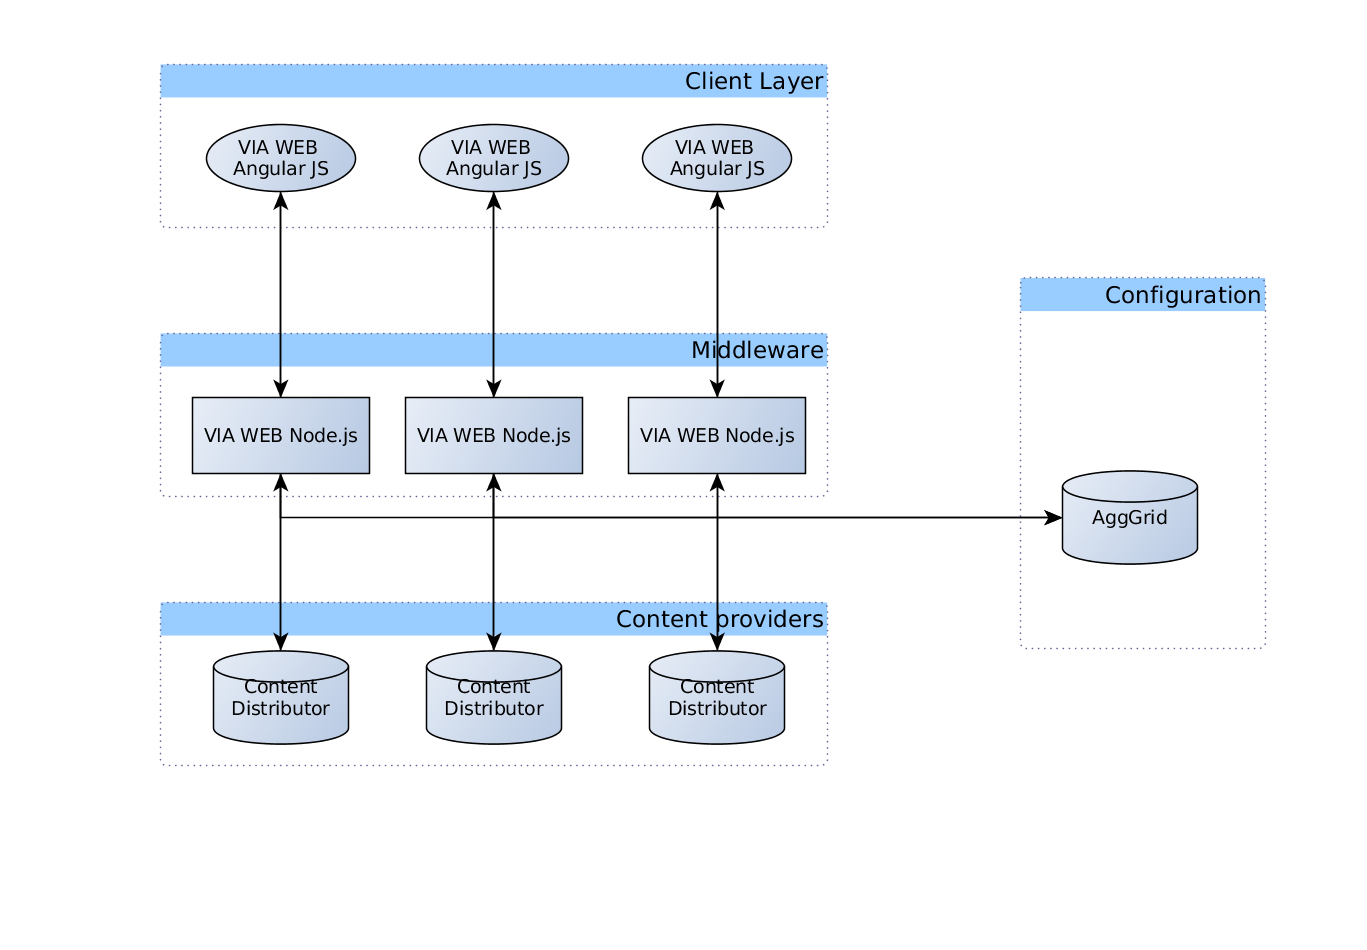
\includegraphics[width=\textwidth]{images/thesis_global_architecture_existing.png}
    \caption{Global architecture overview}
    \label{fig:arch_overview}
\end{figure}


The WEB Angular.js is a web application developed using Javascript, HTML, CSS framework and Model View Controller pattern. In the system, it is indicated as a client application. It communicates with the middleware server through REST services based on HTTP protocol. The client has several components: Controllers, Managers, and Services. 

The contollers validate the user data, invoke corresponding managers, and render data to the view objects represented by HTML pages. The managers are implemented using Facade pattern\cite{DesignPatterns}. They hold and manage services, construct View Model Objects from service responses, and send them back to the controllers. 

The services are the communication layer between the client application and the middleware server. They communicate via REST protocol based on HTTP protocol. This brings flexibility to the architecture and makes components loosely coupled.
% [describe why it is good?]. 

The WEB Node.js is a middleware server. It has several functions:

\begin{itemize}
	\item serves as a data aggregator and security point
	\item translates requests from the client application to the format understandable by the metadata server or content distributors
	\item gathers data from the content distributors
	\item builds data model objects and sends them as JSON entities to the client application.
\end{itemize}

Content servers (content distributors) are customer servers. They are the main sources of information that need to be presented by the client application. They can be represented, for example, by the movie entities or music distributors.

The metadata server is the company-developed server that stores and processes auxiliary and configurational information. The requests can be: 

\begin{itemize}
	\item Data aggregation - required for analytical purposes
	\item User action logs 
	\item User settings - specific user settings, for example, watch history for movie entities
	\item Client and middleware configuration
\end{itemize} 

The interaction between components can be described as follows: the client application initiates the process by sending requests to the middleware server. The middleware server then redirects requests to the underlying servers (content distributors or metadata server), builds data model objects, and sends them to the client application. The client request can be one of two types, configurational or data demand. If the request is configurational, the middleware server redirects it to the metadata server; otherwise, it redirects the request to the content server. The middleware supports the local cache and caches every response that is not associated with the user session. The message diagram between architecture components is depicted on figure \ref{fig:arch_uml}.


\begin{figure}[h]
\begin{center}

	\resizebox{1.0\textwidth}{0.8\textwidth} {

	\begin{sequencediagram}
	\newthread[white]{cl}{Client}
	\newinst[1.7]{mw}{Middleware}
	\newinst{lc}{Local Cache}
	\newinst[1.9]{ms}{Metadata Server}
	\newinst[1.3]{cs}{Content Server}

	\begin{call}{cl}{First request}{mw}{Response}

		\begin{call}{mw}{Create new session}{ms}{Session ID}
		\end{call}

		\begin{call}{mw}{Cache Session}{lc}{}
		\end{call}

		\begin{call}{mw}{Get content locator}{ms}{URL}
		\end{call}

		\begin{call}{mw}{Cache Locator}{lc}{}
		\end{call}

	\end{call}

	\begin{call}{cl}{GET Request}{mw}{GET Response}
		
		\begin{call}{mw}{Check Local Cache}{lc}{}
		\end{call}

		\begin{sdblock}{alt}{if data in cache}
			\begin{call}{mw}{Send response to Client}{cl}{}
			\end{call}
			\begin{sdblock}{else}{}
				\begin{call}{mw}{Request Content}{cs}{Response}
				\end{call}
				\begin{call}{mw}{Cache content}{lc}{}
				\end{call}
			\end{sdblock}
		\end{sdblock}


	\end{call}

	\end{sequencediagram}
	}

\end{center}
\caption{Sequence Diagram of message exchanging}
\label{fig:arch_uml}
\end{figure}

\subsection{Model objects}

In order to understand the existing architecture several definitions should be introduced: Data model object, View Model Object and Application model object.

The data from the content servers differ from one another; as a result, the structure for representing content server objects should be generated dynamically. The asset from the content distributor that has a dynamic structure is called \textit{Data Model Object}(DMO). For example, the DMO can represent information about videos, music, or any other entities. The DMO is generated by the DMO builders from JSON by the middleware server.

The middleware server sends DMOs to the client application. The client application gathers several DMOs and constructs a \textit{View Model Object}(VMO). This object is then presented to the users as a view asset. As a result, the VMO can be defined as a set of data model objects. The VMO is constructed for each HTML page. 

Each content distributor has a set of assets called \textit{Application Model Object}(AMO). Therefore, the application model object is the array of View Model Objects. The AMO represents the information and objects that can be fetched from the single content server.


\subsection{Middleware server architecture}

The middleware server is developed using server side Javascript language and asynchronous server Node.js \cite{Nodejs}. The server is developed using Model View Controller (MVC) pattern and communicates with other components through REST services. As a result, the server components are loosely coupled with each other which gives great flexibility in changing and replacing components and simplifies testing. 

The middleware contains the following components: Controllers, Managers, Services, Configuration and Data Model Object builders. The interraction between components is presented in figure \ref{fig:ms_req}.

\begin{figure}[h]
\begin{center}

	\resizebox{1.0\textwidth}{0.7\textwidth} {

	\begin{sequencediagram}
	\newthread[white]{cl}{Client}
	\newinst[1.7]{cntr}{Controller}
	\newinst[1.3]{mgr}{Manager}
	\newinst[1.3]{lc}{Local Cache}
	\newinst[1.3]{serv}{Service}
	\newinst[1.3]{es}{External Server}

	\begin{call}{cl}{Configuration request}{cntr}{Response}

		\begin{call}{cntr}{Invoke configuation manager}{mgr}{Response Data}
			\begin{call}{mgr}{Check Session key}{lc}{Cache Response}\end{call}
			\begin{sdblock}{alt}{if session key not in cache}
				\begin{call}{mgr}{Get session key using UUID}{serv}{Session key}
					\begin{call}{serv}{Session key request}{es}{Server response}
					\end{call}
				\end{call}
			\end{sdblock}
			\begin{call}{mgr}{Call data service}{serv}{JSON Data}
				\begin{call}{serv}{Call REST API}{es}{JSON data}
				\end{call}
			\end{call}
			\begin{call}{mgr}{Cache response}{lc}{}
			\end{call}
			\begin{call}{mgr}{Make DMO}{mgr}{DMO}\end{call}
		\end{call}

	\end{call}

	\end{sequencediagram}
	}

\end{center}
\caption{Sequence Diagram of Middleware Server Request Process}
\label{fig:ms_req}
\end{figure}

The controllers accept requests from clients. They validate user data and invoke corresponding managers.

The middleware server managers are similar to the client application managers: they implement facade pattern, aggregate multiple services, and redirect requests to them. They also gather the data from services and build immutable Data Model Objects (DMOs). These DMOs are sent back to the client as responses. The workflow of managers is depicted in figure \ref{fig:via_manager}.

\begin{figure}[h]
    \centering
	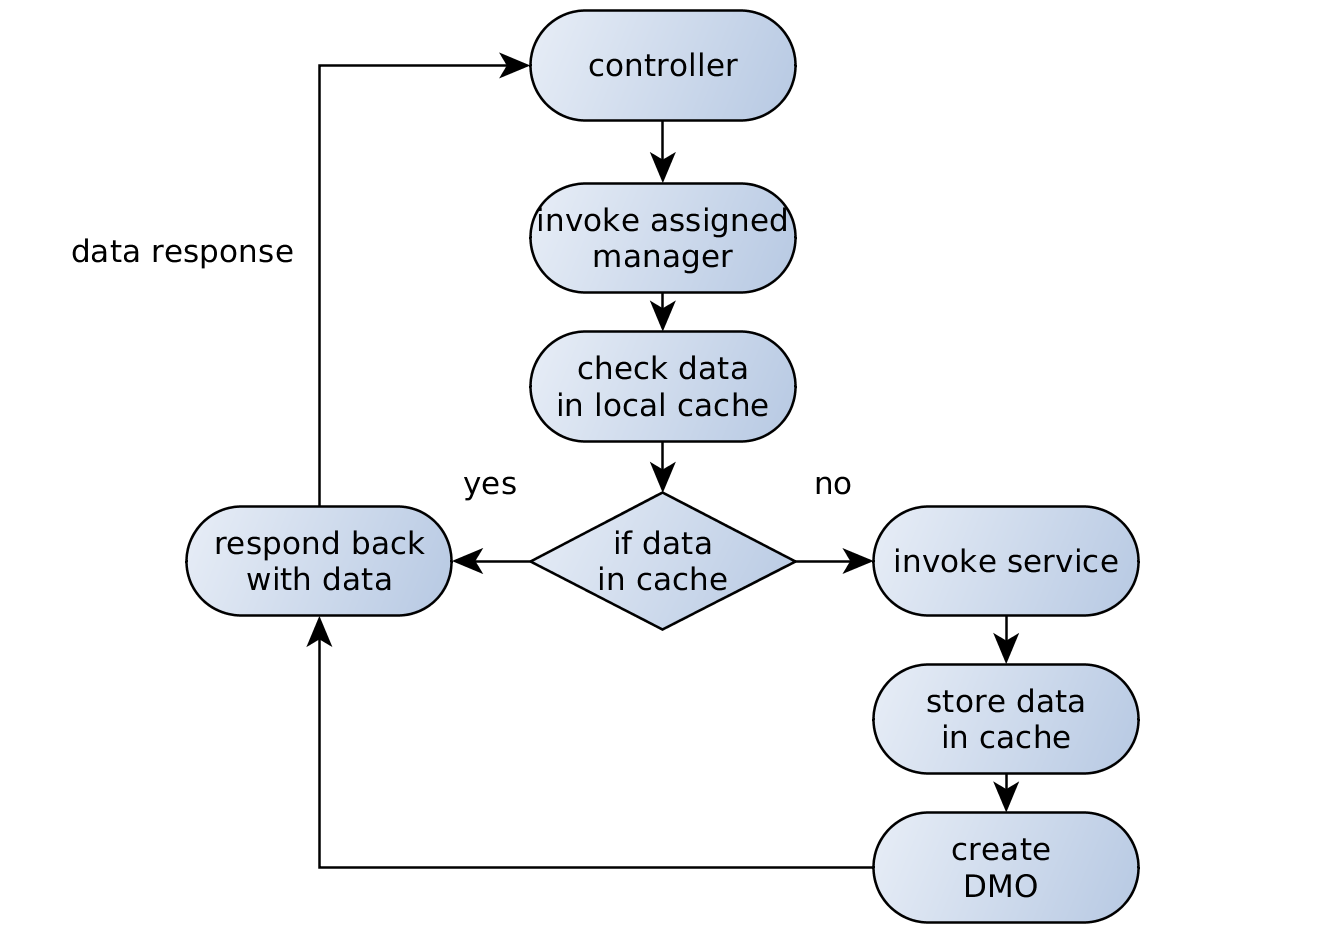
\includegraphics[width=\textwidth]{images/via_manager_1.png}
    \caption{Manager workflow}
    \label{fig:via_manager}
\end{figure}

The middleware services communicate with metadata and content servers. They aggregate the cache layer and react according to the following algorithm: first they check if the data is presented in the local cache; if the service observes cache hit, it will check the object's time to live (TTL) and send the corresponding object back to the manager. On the other hand, if a cache miss occurs, it will send the GET request through the REST protocol to the metadata server or content server, store the response locally for predefined period of time, and send it back to the manager. The workflow of services is presented in figure \ref{fig:via_service}. The time to live is the time (usually specified in seconds) that represents how long the object can be considered fresh without hitting persistence layer.


\begin{figure}[h]
    \centering
	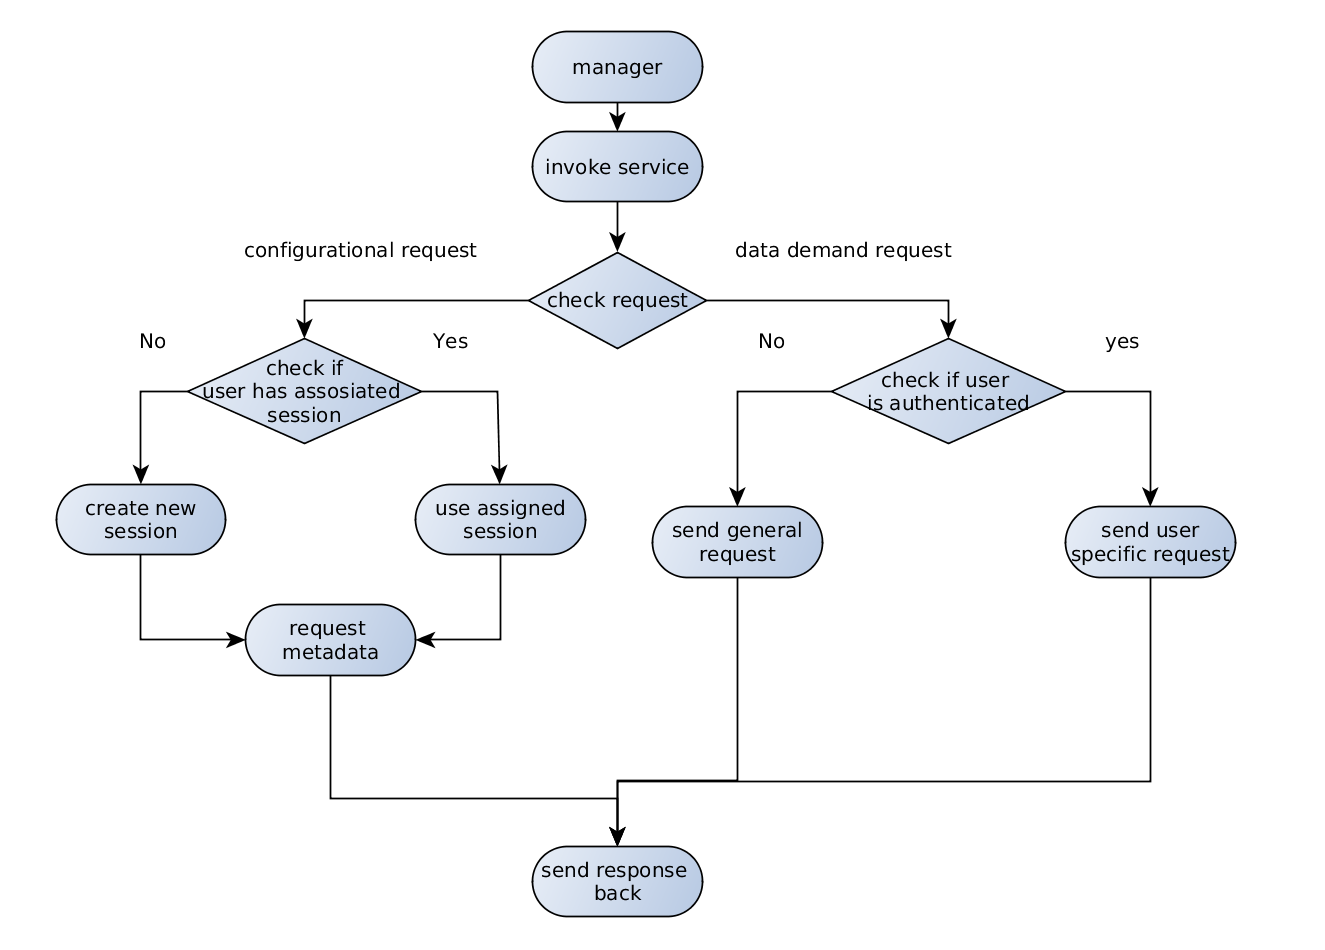
\includegraphics[width=\textwidth]{images/via_service_1.png}
    \caption{Service workflow}
    \label{fig:via_service}
\end{figure}


The client application can make two types of requests: configurational and data demand requests.
The configurational request can have the following purposes:

\begin{itemize}
	\item Provide configuration parameters for both middleware server and client application
	\item Write user activy
	\item Check the health of metadata server
	\item Get Content Server url
	\item User settings and preferences
	\item Analytics
\end{itemize}


The data demand request is a request to the content servers. Since content servers are customer servers, the response doesn't have predefined structure and can have any structure specified by customer service. 

The control flow can be described as follows: the controller receives a request from the client application, validates the data in the request, and redirects it to the assigned manager. The middleware server manager invokes the corresponding service (for example, communications layers). When the client application makes a data demand request, the manager invokes content service that redirects the request to the assigned content server. The response is then stored in the cache, translated into Data Model Object, and transferred back to the client in JSON format. The DMO builders are in charge of translating JSON data into persistent Data Model Objects. For every DMO, there is an assigned manager and service. For example, if the content server responds with a video object, there will be VideoManager and VideoService components.

\subsection{Session management}

The security layer, which is represented by the session management, is responsible for a communication process between the middleware server and inner servers (metadata server and content distributors).

The application session consists of two parts: 

\begin{itemize}
	\item client session
	\item middleware session
\end{itemize}

The purpose of sessions is to distinct between users and provide corresponding analytics to the customers.

The client session is represented by the unique session identifier (UID) and the browser's ID (the string that identifies browser version in the internet). These parameters are generated by the middleware server and transferred to the client through the \textit{set-cookie} header. The browser remembers the data and sends it back with every request in the \textit{cookie} header.


The session is generated per client when he makes the initial request. It contains the metadata session key and the user session, if the user is authenticated. The metadata session is obtained by making a request to the metadata server. The middleware server sends the application key parameter, which is specified in the configuration file and browser ID. The metadata server validates the application key and generates a new session for the middleware server. The middleware server assigns this session to the client and stores it in local memory. The client sends the unique session with each request to the middleware server. The middleware server retrieves the metadata session from the client's request. Using this session, the middleware server can make configurational requests to the metadata server. The sequence diagram of session management is presented in figure \ref{fig:arch_sess_uml}. The application key is given by the system administrator to each middleware server. The browser ID can be any string and does not have validation rules.

\begin{figure}[h]
\begin{center}

	\resizebox{1.1\textwidth}{0.5\textwidth} {

	\begin{sequencediagram}
	\newthread[white]{cl}{Client}
	\newinst[1.5]{md}{Middleware server}
	\newinst[3.0]{mt}{Metadata server}

	\begin{call}{cl}{RequestSession}{md}{Client session}

		\begin{call}{md}{GenerateSessionId}{md}{ClientSessionId} \end{call}
		\begin{call}{md}{GenerateBrowserId}{md}{BrowserId} \end{call}
		\begin{call}{md}{RequestMetadataSession}{mt}{MetadataSession} 
			\begin{call}{mt}{Validate Data}{mt}{}\end{call}
		\end{call}

	\end{call}

	\end{sequencediagram}
	}

\end{center}
\caption{Sequence Diagram of Middleware Session generation}
\label{fig:arch_sess_uml}
\end{figure}


\subsection{Drawbacks of the current architecture}

After careful examination, two categories of problems were defined: client application drawbacks and middleware server drawbacks. 

In order to render the page, the client needs to generate a view model object. The VMO contains several data model objects. The client makes a request for every DMO, aggregates the response, generates VMO from DMOs, and renders it to the HTML view. The drawback is that the client has to make several HTTP requests in order to generate a single VMO. It would be better for the client to make a request for VMO instead of DMO. This approach has some advantages: the client will make less HTTP requests which will increase the performance by reducing the latency and simplify the client's logic considering the client will not be required to generate VMOs from DMOs. 

Another problem with the current client implementation is that it is not generic. If a new content server is introduced, a lot of code would have to be modified on the client side in order to implement the new logic. To solve this, the client can maintain the caching layer that will cache VMOs from the responses. 

Additional complications occur when the client implements MVC pattern, which produces duplication with the middleware server. This approach increases the complexity of the system, since the developers would have to support both the client and the middleware MVC applications. To rectify this, we can simplify the client application and assign two tasks to it: caching and rendering VMOs.

On the middleware side, the DMOs are not generic. The purpose of the middleware server is to serve as a transparent layer, but without dynamic DMO generation a lot of code has to be changed when the new content server is introduced.

The middleware cache can be replaced by the Content Delivery Network (CDN). The middleware caches only information that is common for every user. This work can be done by the CDN edge servers. These will decrease the middleware complexity and decrease the cost of maintaining middleware server.


\newpage
